\documentclass[11pt]{article}
\usepackage{geometry}
\usepackage{coling2020}
\usepackage{times}
\usepackage{url}
\usepackage{latexsym}
\usepackage{microtype}
\usepackage{amssymb}
\usepackage[cmex10]{amsmath}
\usepackage{amsmath,amssymb,amsfonts}
\usepackage{comment}
\usepackage{graphicx}
\graphicspath{{Figures/EPS/}{figures/}}
\usepackage[usestackEOL]{stackengine}
\usepackage{array, tabularx, booktabs, multicol, multirow, supertabular}
\usepackage{tabulary}
\usepackage{pdfpages}
\usepackage{color}
\usepackage[misc]{ifsym}
\usepackage{enumerate}
\usepackage[shortlabels]{enumitem}
%\usepackage[linesnumbered,ruled,vlined]{algorithm2e}
\usepackage[ruled,vlined]{algorithm2e}
\usepackage{algorithmic}
\usepackage[hidelinks, bookmarks=false]{hyperref}
\usepackage{makecell}
\usepackage{calc}
\usepackage{times}
\usepackage{latexsym}
\usepackage{longtable}


\hyphenation{an-aly-sis}
\hyphenation{an-aly-ses}
\colingfinalcopy 

\newcommand*{\affaddr}[1]{#1} % No op here. Customize it for different styles.
\newcommand*{\affmark}[1][*]{\textsuperscript{#1}}

\DeclareMathOperator*{\argmin}{\arg\!\min}
\DeclareMathOperator*{\argmax}{\arg\!\max}



\title{Workshop on LaTex for Academic, Technical, and Professional Writing}

\author{Student (Student ID:  ) \\
  Department of Computer Science and Engineering \\
  \affaddr{University of Chittagong, Chittagong, Bangladesh}\\
  {\tt name@gmail.com (\Letter)} \\
}



\begin{document}
%
\includepdf[pages=-]{./coverpage/CoverPage}
\maketitle
%\thispagestyle{plain}
\pagestyle{plain}

\section{Inline Text Manipulation}
\label{ref:inlineText}
Microblog platforms such as ``twitter", \emph{sina weibo}, etc. are rapidly moving towards a platform for $\mbox{sample text}$ user-generated information production and consumption. Among the several microblog services, \#twitter has become the most popular. The real-time nature of twitter plays an {\color{red} important role during a disaster period}, such as earthquakes, \textbackslash{wildfires}, and so on. This is because the user-generated twitter posts during such events might be useful to serve the situational information needs ($\approx$ 59\% \& 89\%). To\_use\_underscore it is $X_{2}$ $4^{th}$ \textcopyright2021.
%{\color{blue} colored text}
%{\color[HTML]{38B25A}


\section{Itemize and Enumerate}
\label{ref:itemize}

\subsection{The General Type of Itemize}
\begin{itemize}
\item Explore the image.
\item Explore the text.
\item Expore the video.
\item Explore the sound.
\item Create the multimodal data.
\end{itemize}

\subsection{Using the Special Symbol for Item Label}
\begin{itemize}
\item[--] Explore the image.
\item[*] Explore the image.
\item[$\diamond$] Explore the text.
\item[$\blacktriangleright$] Expore the video.
\item[$\star$] Explore the sound.
\item[$\blacksquare$] Create the multimodal data.
\end{itemize}


\subsection{Numbered Type Itemize}
\begin{enumerate}
\item Explore the image.
\item Explore the text.
\item Expore the video.
\item Explore the sound.
\item Create the multimodal data.
\end{enumerate}

\subsection{English alphabetic Type Itemize (Lowercase)}
\begin{enumerate}[A]
\item Explore the image.
\item Explore the text.
\item Expore the video.
\item Explore the sound.
\item Create the multimodal data.
\end{enumerate}


\subsection{Roman Numbered Type Itemize (Lowercase)}
\begin{enumerate}[i]
\item Explore the image.
\item Explore the text.
\item Expore the video.
\item Explore the sound.
\item Create the multimodal data.
\end{enumerate}

\subsection{Roman Numbered Type Itemize (Uppercase)}
\begin{enumerate}[I]
\item Explore the image.
\item Explore the text.
\item Expore the video.
\item Explore the sound.
\item Create the multimodal data.
\end{enumerate}

\subsection{Reducing Space between Items}
\begin{enumerate}[nosep]
\item Explore the image.
\item Explore the text.
\item Expore the video.
\item Explore the sound.
\item Create the multimodal data.
\end{enumerate}

\subsection{Reducing Space between Items and Provide Special Item Label}
\begin{enumerate}[nosep, label=*]
\item Explore the image.
\item Explore the text.
\item Expore the video.
\item Explore the sound.
\item Create the multimodal data.
\end{enumerate}

\subsection{Reducing Space between Items and Provide Romanized Item Label}
\begin{enumerate}[nosep, label=\roman*]
\item Explore the image.
\item Explore the text.
\item Expore the video.
\item Explore the sound.
\item Create the multimodal data.
\end{enumerate}


\subsection{Reducing Space between Items and Provide Numeric Item Label}
\begin{enumerate}[nosep, label=\arabic*]
\item Explore the image.
\item Explore the text.
\item Expore the video.
\item Explore the sound.
\item Create the multimodal data.
\end{enumerate}


\subsection{Adding Specific Character with Each Numeric Item Label}
\begin{enumerate}[nosep, label=B\arabic*]
\item Explore the image.
\item Explore the text.
\item Expore the video.
\item Explore the sound.
\item Create the multimodal data.
\end{enumerate}


\subsection{Numeric Item Label with Bracket}
\begin{enumerate}[nosep, label=(\arabic*)]
\item Explore the image.
\item Explore the text.
\item Expore the video.
\item Explore the sound.
\item Create the multimodal data.
\end{enumerate}


\subsection{Numeric Item Label with Dot}
\begin{enumerate}[nosep, label=\arabic*.]
\item Explore the image.
\item Explore the text.
\item Expore the video.
\item Explore the sound.
\item Create the multimodal data.
\end{enumerate}


\subsection{Alphabetic Item Label with dot}
\begin{enumerate}[nosep, label=\alph*.]
\item Explore the image.
\item Explore the text.
\item Expore the video.
\item Explore the sound.
\item Create the multimodal data.
\end{enumerate}


\subsection{Alphabetic Item Label with dot}
\begin{enumerate}[nosep, label=\Alph*.]
\item Explore the image.
\item Explore the text.
\item Expore the video.
\item Explore the sound.
\item Create the multimodal data.
\end{enumerate}

\subsection{Romanized Item Label with dot}
\begin{enumerate}[nosep, label=\roman*.]
\item Explore the image.
\item Explore the text.
\item Expore the video.
\end{enumerate}

\subsection{Romanized Item Label with dot}
\begin{enumerate}[nosep, label=\Roman*.]
\item Explore the image.
\item Explore the text.
\item Expore the video.
\item Explore the sound.
\end{enumerate}



\section{Mathematical Equation and Expression}
\label{ref:equation}
\begin{equation}
e_{t}=h_{t}w_{a}
\label{eqn:sampleEqn}
\end{equation}

\begin{equation*}
a_{t}  = \frac{\exp(e_{t})}{\sum^{T}_{i=1}\exp(e_{i})}
\end{equation*}

\begin{equation*}
v={\sum^{T}_{i=1} a_{i}h_{i}}
\end{equation*}

\begin{equation*}
P(m^{(i)},n^{(i)}) = \sum^{k}_{j=1} 1\{n^{(i)}=j\} \log(n_{j}^{\thicksim(i)})
\end{equation*}


\begin{equation*}
\begin{split}
\mbox{Combined Span} = &Span[index[1]] \cup \\  
                       &Span[index[1]] \cup \\
                       &Span[index[1]]
\end{split}
\end{equation*}


\begin{equation*}
\begin{split}
R_j: & \ \mbox{if}\ x_1\ \mbox{is}\ A_{j1}\ \mbox{and/or}\ ........\ x_n\ \mbox{is}\ A_{jn}\\
	 & \ \mbox{then}\ Class=C_j, \ \ \ j=1,......,N
\end{split}
\end{equation*}

%$\underset{f_i}{argmax} ((h_i, f_i))$

\subsection{Nested LSTMs (NLSTMs)}
\label{ref:nestedLSTMs}
Nowadays, LSTM based deep learning models are the most popular choice for sequential tasks. In our model, we employ the state-of-the-art nested LSTMs (NLSTMs) model where the LSTM memory cells selectively read and write necessary long-term information through accessing their inner memory. Though LSTM is employing $c_{t}^{outer}={f_{t}}\odot{c_{t-1}}+{i_{t}}\odot{g_{t}}$ to estimate it's outer memory cell value, NLSTMs use the concatenation $({f_{t}}\odot{c_{t-1}},{i_{t}}\odot{g_{t}})$ as an input to an inner LSTM (or NLSTM) memory cell, and set $c_{t}^{outer}=h_{t}^{inner}$. Such mechanism helps the NLSTMs to operate on longer time-scales thus capture the contextual information effectively.


\section{Figure Inclusion}
\label{ref:figure}

\begin{figure}[!htb]
\centering
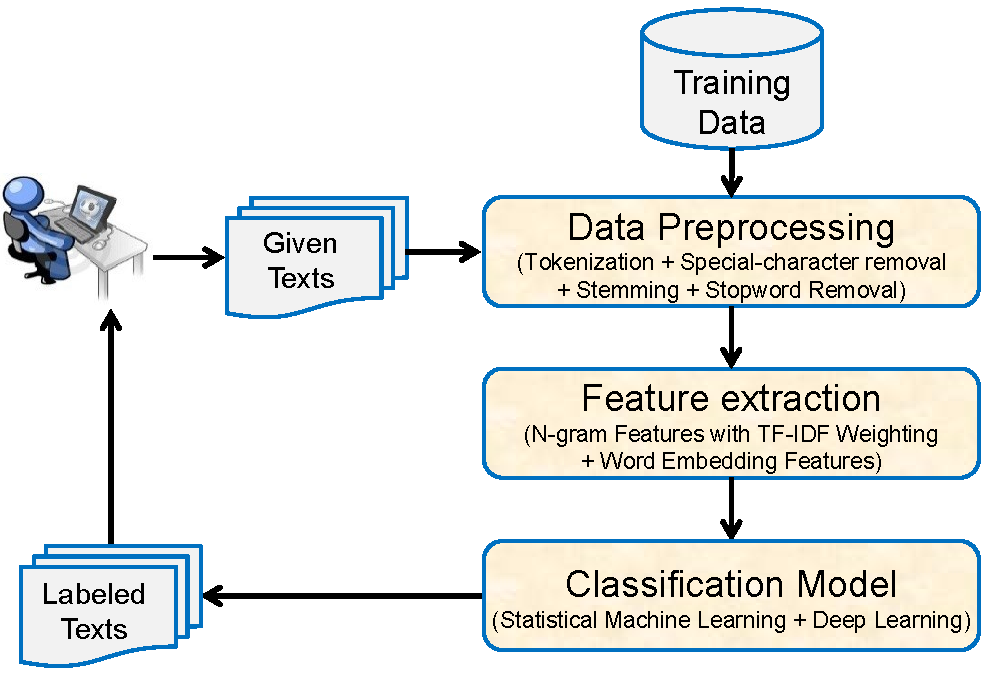
\includegraphics[width=0.65\linewidth]{overview.pdf}
\caption{Proposed framework.}
\label{fig:overview}
\end{figure}


\begin{figure}[!htb]
\centering
\begin{tabular}{cp{0.5cm}c}
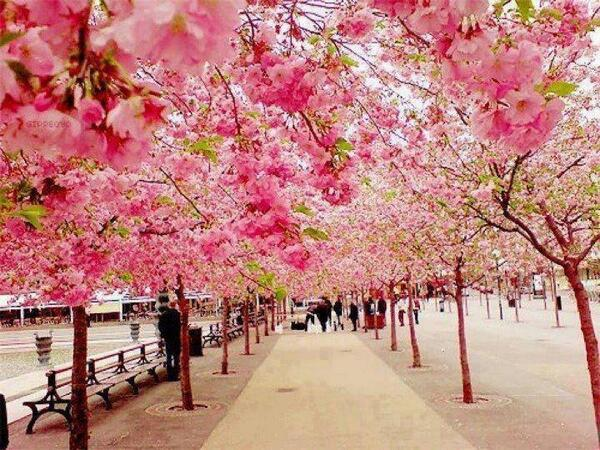
\includegraphics[width=0.4\textwidth]{Pos4.jpg}
&
&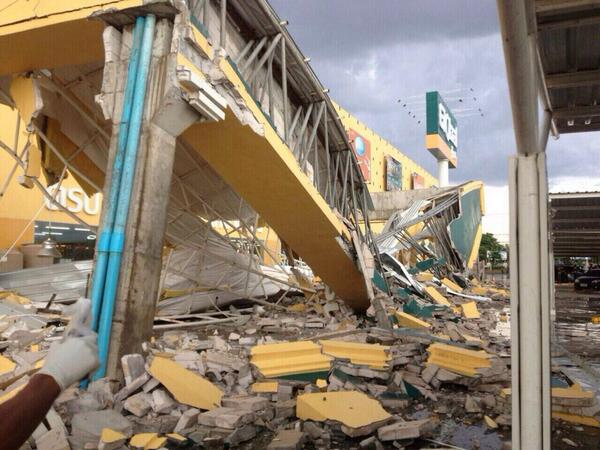
\includegraphics[width=0.4\textwidth]{Neg3.jpg}
\end{tabular}
\caption{Sample of positive (left) and negative (right) sentiment bearing images.}
\label{Fig:sampleImage}
\end{figure}

\section{Table}
\label{ref:table}
Now, we illustrate the different types of tables. See the long table illustration from here~\url{https://www.overleaf.com/latex/examples/a-longtable-example/xxwzfxkxxjmc}. Other types of tables are illustrated below:

\begin{table}[!h]
\centering
\caption{A sample table.}
\begin{tabular}{|c|c|l|c|} 
\hline
\textbf{Col1} & \textbf{Col2} & \multicolumn{1}{c|}{\textbf{Col3}} & \textbf{Col4} \\
\hline
1 & 6 & 87837 & --\\ 
\hline
2 & 7 & 78 & 5415 \\
\hline
3 & 545 & 778 & 7507 \\
\hline
4 & 545 & 18744 & 7560 \\
\hline
\end{tabular}
\end{table}


\begin{table}[!htb]
\renewcommand{\tabcolsep}{2mm} %6.5mm
\renewcommand{\arraystretch}{1.1}
\centering
\begin{tabular} {lc}
\toprule
\multicolumn{1}{c}{Team Name} &F1-Score \\ 
\midrule
HITSZ-HLT9 (1st) &0.7083028253 \\
hitmi\&t (3rd)   &0.6984762534\\
IITK\@Detox (9th)	&0.6895352367\\
\textbf{CSECUDSG (21st)}  &	\textbf{0.6795264755} \\
mnfourka (45th)      &0.6581458018\\
ST\_TSResearch (64th) &0.6133591537  \\	
\bottomrule
\end{tabular}
\caption{Comparative performance analysis.}
\label{tab:result1}
\end{table}


\begin{table}[h!]
\centering
\caption{Comparative performance analysis against the state-of-the-art.}
\label{tab:top5ResultTRECIS}   
\begin{tabular}{lcccc}
\toprule
\midrule
\multicolumn{1}{c}{ \multirow{2}[3]{*}{Methods} } & \multicolumn{4}{c}{Any-Type (Micro Avg.)}\\
\cmidrule{2-5} &Precision &Recall &\textbf{F1 Score} &Accuracy\\
\midrule
Proposed Method  &0.4504 &\textbf{1.0000} &\textbf{0.6210} &\textbf{0.4504}\\
\midrule
\multicolumn{5}{l}{\textit{Top 5 Performing Teams in TRECIS-2018}}\\
\midrule
cbnuS2  	     &\textbf{0.4559} &0.7780 &0.5749 &0.4213 \\
KDEIS4\_DM       &0.3914 &0.9856 &0.5603 &0.3908\\
umdhcilfasttext  &0.4534 &0.7260 &0.5582 &0.4022\\
\midrule
Participant Median &0.3978 &0.6165 &0.4775 &0.3385\\
\bottomrule
\end{tabular}
\end{table}



\section{Pseudocode/Algorithm Inclusion}
\label{ref:algorithm}

\begin{algorithm}[H]
\SetAlgoLined
\KwIn{Input:\\}
\KwOut{Output:\\}
\KwResult{Write here the result }
 initialization\;
 \While{While condition}{
  instructions\;
  \eIf{condition}{
   instructions1\;
   instructions2\;
   }{
   instructions3\;
  }
 }
\caption{How to write algorithms}
\end{algorithm}


\begin{algorithmic}
\STATE $i\gets 10$
\IF {$i\geq 5$} 
        \STATE $i\gets i-1$
\ELSE
        \IF {$i\leq 3$}
                \STATE $i\gets i+2$
        \ENDIF
\ENDIF 
\end{algorithmic}


\section{External PDF Pages Inclusion}
\label{ref:pdf}



\section{Footnote and Citation/References}
\label{ref:citation}

Some sample texts to illustrate the use of footnote\footnote{Footnte sometimes used as a provider of additional information}. Also we can use the url reference as footnote\footnote{https://github.com/nowshedcu/Personality-Traits-Detection-in-Bangla}.
\\

To add a reference of a research paper, we need to collect bibtex from google scholar and put this bibtex in the *.bib file. Then, we can add the reference as follows:~\cite{moniz2017nested}~\cite{kopka1995guide}.

%
\section{Miscellaneous}
\label{ref:miscellaneous}
we publicly release the dataset for future research purposes at the following link: \url{https://git.io/JkW6V} or use the expanded URL\footnote{https://github.com/nowshedcu/Personality-Traits-Detection-in-Bangla}


\section{Illustration of Section}
\label{ref:sectionLabel}

\subsection{This is Subsection:}
\label{ref:subsection}

\subsubsection{This is Subsubsection:}
\label{ref:subsubsection}

%

\section{Domain Specific Template Manipulation}
\label{ref:template}

IEEE Template~\url{https://www.ieee.org/conferences/publishing/templates.html}.


% include your own bib file like this:
\bibliographystyle{coling}
\bibliography{reference}

\end{document}
